%%%% Paramétrage du TD %%%%
\def\xxactivite{ \ifprof \normalsize{TD 5 -- Corrigé } \else  \ifcolle Colle \else TD 5\fi \fi} % \normalsize \vspace{-.4cm}
\def\xxauteur{\textsl{Xavier Pessoles}}


\def\xxnumchapitre{Chapitre 1 \vspace{.2cm}}
\def\xxchapitre{\hspace{.12cm} Approche énergétique}

\def\xxcompetences{%
\vspace{-.5cm}
\footnotesize{
\textsl{%
\textbf{Savoirs et compétences :}\\
\vspace{-.2cm}
\begin{itemize}[label=\ding{112},font=\color{ocre}] 
\item Mod2.C18.SF1 : Déterminer l’énergie cinétique d’un solide, ou d’un ensemble de solides, dans son mouvement par rapport à un autre solide.
\item Res1.C1.SF1 : Proposer une démarche permettant la détermination de la loi de mouvement.
%\item Mod1.C5.SF2 : Déterminer la puissance des actions mécaniques extérieures à un solide ou à un ensemble de solides, dans son mouvement rapport à un autre solide.
%\item Mod1.C5.SF3 : Déterminer la puissance des actions mécaniques intérieures à un ensemble de solides.
\end{itemize}}}}


\def\xxtitreexo{RobuROC 6 : plate-forme d’exploration tout terrain\ifnormal $\star$ \else \fi \iftdifficile $\star\star\star$ \else \fi }
\def\xxsourceexo{\hspace{.2cm} \footnotesize{Concours Commun Mines Ponts 2009}}

\def\xxfigures{
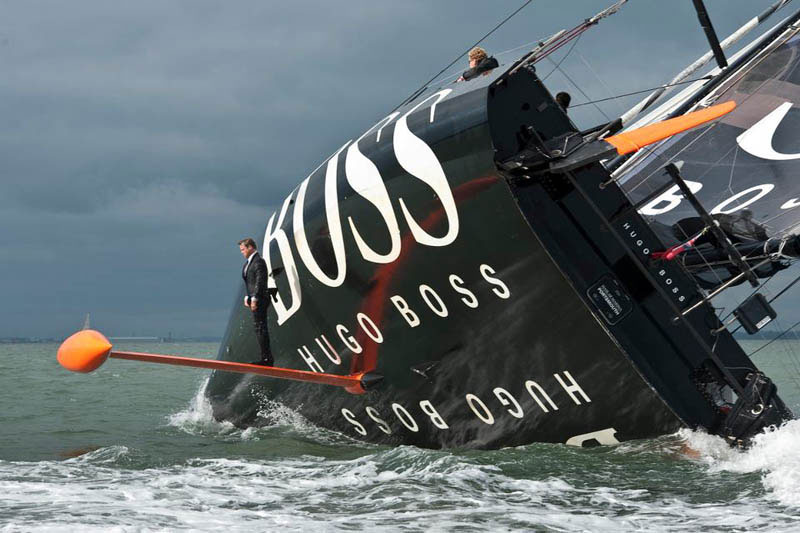
\includegraphics[width=.7\textwidth]{fig_00}
}%figues de la page de garde


\iflivret
\pagestyle{empty}


%%%%%%%% PAGE DE GARDE COURS
\ifcours
% ==== BANDEAU DES TITRES ==== 
\begin{tikzpicture}[remember picture,overlay]
\node at (current page.north west)
{\begin{tikzpicture}[remember picture,overlay]
\node[anchor=north west,inner sep=0pt] at (0,0) {\includegraphics[width=\paperwidth]{\thechapterimage}};
\draw[anchor=west] (-2cm,-8cm) node [line width=2pt,rounded corners=15pt,draw=ocre,fill=white,fill opacity=0.6,inner sep=40pt]{\strut\makebox[22cm]{}};
\draw[anchor=west] (1cm,-8cm) node {\huge\sffamily\bfseries\color{black} %
\begin{minipage}{1cm}
\rotatebox{90}{\LARGE\sffamily\textsc{\color{ocre}\textbf{\xxnumpartie}}}
\end{minipage} \hfill
\begin{minipage}[c]{14cm}
\begin{titrepartie}
\begin{flushright}
\renewcommand{\baselinestretch}{1.1} 
\Large\sffamily\textsc{\textbf{\xxpartie}}
\renewcommand{\baselinestretch}{1} 
\end{flushright}
\end{titrepartie}
\end{minipage} \hfill
\begin{minipage}[c]{3.5cm}
{\large\sffamily\textsc{\textbf{\color{ocre} \discipline}}}
\end{minipage} 
 };
\end{tikzpicture}};
\end{tikzpicture}
% ==== FIN BANDEAU DES TITRES ==== 


% ==== ONGLET 
\begin{tikzpicture}[overlay]
\node[shape=rectangle, 
      rounded corners = .25 cm,
	  draw= ocre,
	  line width=2pt, 
	  fill = ocre!10,
	  minimum width  = 2.5cm,
	  minimum height = 3cm,] at (18.3cm,0) {};
\node at (17.7cm,0) {\rotatebox{90}{\textbf{\Large\color{ocre}{\classe}}}};
%{};
\end{tikzpicture}
% ==== FIN ONGLET 


\vspace{3.5cm}

\begin{tikzpicture}[remember picture,overlay]
\draw[anchor=west] (-2cm,-6cm) node {\huge\sffamily\bfseries\color{black} %
\begin{minipage}{2cm}
\begin{center}
\LARGE\sffamily\textsc{\color{ocre}\textbf{\xxactivite}}
\end{center}
\end{minipage} \hfill
\begin{minipage}[c]{15cm}
\begin{titrechapitre}
\renewcommand{\baselinestretch}{1.1} 
\Large\sffamily\textsc{\textbf{\xxnumchapitre}}

\Large\sffamily\textsc{\textbf{\xxchapitre}}
\vspace{.5cm}

\renewcommand{\baselinestretch}{1} 
\normalsize\normalfont
\xxcompetences
\end{titrechapitre}
\end{minipage}  };
\end{tikzpicture}
\vfill

\begin{flushright}
\begin{minipage}[c]{.3\linewidth}
\begin{center}
\xxfigures
\end{center}
\end{minipage}\hfill
\begin{minipage}[c]{.6\linewidth}
\startcontents
%\printcontents{}{1}{}
\printcontents{}{1}{}
\end{minipage}
\end{flushright}

\begin{tikzpicture}[remember picture,overlay]
\draw[anchor=west] (4.5cm,-.7cm) node {
\begin{minipage}[c]{.2\linewidth}
\begin{flushright}

\includegraphics[width=2cm]{logoCC}
\end{flushright}
\end{minipage}
\begin{minipage}[c]{.2\linewidth}
\textsl{\xxauteur} \\
\textsl{\classe}
\end{minipage}
 };
\end{tikzpicture}

\newpage
\pagestyle{fancy}

%\newpage
%\pagestyle{fancy}

\else
\fi
%% FIN PAGE DE GARDE DES COURS

%%%%%%%% PAGE DE GARDE TD
\iftd
%\begin{tikzpicture}[remember picture,overlay]
%\node at (current page.north west)
%{\begin{tikzpicture}[remember picture,overlay]
%\draw[anchor=west] (-2cm,-3.25cm) node [line width=2pt,rounded corners=15pt,draw=ocre,fill=white,fill opacity=0.6,inner sep=40pt]{\strut\makebox[22cm]{}};
%\draw[anchor=west] (1cm,-3.25cm) node {\huge\sffamily\bfseries\color{black} %
%\begin{minipage}{1cm}
%\rotatebox{90}{\LARGE\sffamily\textsc{\color{ocre}\textbf{\xxnumpartie}}}
%\end{minipage} \hfill
%\begin{minipage}[c]{13.5cm}
%\begin{titrepartie}
%\begin{flushright}
%\renewcommand{\baselinestretch}{1.1} 
%\Large\sffamily\textsc{\textbf{\xxpartie}}
%\renewcommand{\baselinestretch}{1} 
%\end{flushright}
%\end{titrepartie}
%\end{minipage} \hfill
%\begin{minipage}[c]{3.5cm}
%{\large\sffamily\textsc{\textbf{\color{ocre} \discipline}}}
%\end{minipage} 
% };
%\end{tikzpicture}};
%\end{tikzpicture}

%%%%%%%%%% PAGE DE GARDE TD %%%%%%%%%%%%%%%
%\begin{tikzpicture}[overlay]
%\node[shape=rectangle, 
%      rounded corners = .25 cm,
%	  draw= ocre,
%	  line width=2pt, 
%	  fill = ocre!10,
%	  minimum width  = 2.5cm,
%	  minimum height = 2.5cm,] at (18.5cm,0) {};
%\node at (17.7cm,0) {\rotatebox{90}{\textbf{\Large\color{ocre}{\classe}}}};
%%{};
%\end{tikzpicture}

% PARTIE ET CHAPITRE
%\begin{tikzpicture}[remember picture,overlay]
%\draw[anchor=west] (-1cm,-2.1cm) node {\large\sffamily\bfseries\color{black} %
%\begin{minipage}[c]{15cm}
%\begin{flushleft}
%\xxnumchapitre \\
%\xxchapitre
%\end{flushleft}
%\end{minipage}  };
%\end{tikzpicture}

% BANDEAU EXO
\iflivret % SI LIVRET
\begin{tikzpicture}[remember picture,overlay]
\draw[anchor=west] (-2cm,-3.3cm) node {\huge\sffamily\bfseries\color{black} %
\begin{minipage}{5cm}
\begin{center}
\LARGE\sffamily\color{ocre}\textbf{\textsc{\xxactivite}}

\begin{center}
\xxfigures
\end{center}

\end{center}
\end{minipage} \hfill
\begin{minipage}[c]{12cm}
\begin{titrechapitre}
\renewcommand{\baselinestretch}{1.1} 
\large\sffamily\textbf{\textsc{\xxtitreexo}}

\small\sffamily{\textbf{\textit{\color{black!70}\xxsourceexo}}}
\vspace{.5cm}

\renewcommand{\baselinestretch}{1} 
\normalsize\normalfont
\xxcompetences
\end{titrechapitre}
\end{minipage}};
\end{tikzpicture}
\else % ELSE NOT LIVRET
\begin{tikzpicture}[remember picture,overlay]
\draw[anchor=west] (-2cm,-4.5cm) node {\huge\sffamily\bfseries\color{black} %
\begin{minipage}{5cm}
\begin{center}
\LARGE\sffamily\color{ocre}\textbf{\textsc{\xxactivite}}

\begin{center}
\xxfigures
\end{center}

\end{center}
\end{minipage} \hfill
\begin{minipage}[c]{12cm}
\begin{titrechapitre}
\renewcommand{\baselinestretch}{1.1} 
\large\sffamily\textbf{\textsc{\xxtitreexo}}

\small\sffamily{\textbf{\textit{\color{black!70}\xxsourceexo}}}
\vspace{.5cm}

\renewcommand{\baselinestretch}{1} 
\normalsize\normalfont
\xxcompetences
\end{titrechapitre}
\end{minipage}};
\end{tikzpicture}

\fi

\else   % FIN IF TD
\fi


%%%%%%%% PAGE DE GARDE FICHE
\iffiche
\begin{tikzpicture}[remember picture,overlay]
\node at (current page.north west)
{\begin{tikzpicture}[remember picture,overlay]
\draw[anchor=west] (-2cm,-2.25cm) node [line width=2pt,rounded corners=15pt,draw=ocre,fill=white,fill opacity=0.6,inner sep=40pt]{\strut\makebox[22cm]{}};
\draw[anchor=west] (1cm,-2.25cm) node {\huge\sffamily\bfseries\color{black} %
\begin{minipage}{1cm}
\rotatebox{90}{\LARGE\sffamily\textsc{\color{ocre}\textbf{\xxnumpartie}}}
\end{minipage} \hfill
\begin{minipage}[c]{14cm}
\begin{titrepartie}
\begin{flushright}
\renewcommand{\baselinestretch}{1.1} 
\large\sffamily\textsc{\textbf{\xxpartie} \\} 

\vspace{.2cm}

\normalsize\sffamily\textsc{\textbf{\xxnumchapitre -- \xxchapitre}}
\renewcommand{\baselinestretch}{1} 
\end{flushright}
\end{titrepartie}
\end{minipage} \hfill
\begin{minipage}[c]{3.5cm}
{\large\sffamily\textsc{\textbf{\color{ocre} \discipline}}}
\end{minipage} 
 };
\end{tikzpicture}};
\end{tikzpicture}

\iflivret
\begin{tikzpicture}[overlay]
\node[shape=rectangle, 
      rounded corners = .25 cm,
	  draw= ocre,
	  line width=2pt, 
	  fill = ocre!10,
	  minimum width  = 2.5cm,
	  minimum height = 2.5cm,] at (18.5cm,1.1cm) {};
\node at (17.9cm,1.1cm) {\rotatebox{90}{\textsf{\textbf{\large\color{ocre}{\classe}}}}};
%{};
\end{tikzpicture}
\else
\begin{tikzpicture}[overlay]
\node[shape=rectangle, 
      rounded corners = .25 cm,
	  draw= ocre,
	  line width=2pt, 
	  fill = ocre!10,
	  minimum width  = 2.5cm,
%	  minimum height = 2.5cm,] at (18.5cm,1.1cm) {};
	  minimum height = 2.5cm,] at (18.6cm,0cm) {};
\node at (18cm,0cm) {\rotatebox{90}{\textsf{\textbf{\large\color{ocre}{\classe}}}}};
%{};
\end{tikzpicture}

\fi

\else
\fi



\else
\pagestyle{empty}


%%%%%%%% PAGE DE GARDE COURS
\ifcours
% ==== BANDEAU DES TITRES ==== 
\begin{tikzpicture}[remember picture,overlay]
\node at (current page.north west)
{\begin{tikzpicture}[remember picture,overlay]
\node[anchor=north west,inner sep=0pt] at (0,0) {\includegraphics[width=\paperwidth]{\thechapterimage}};
\draw[anchor=west] (-2cm,-8cm) node [line width=2pt,rounded corners=15pt,draw=ocre,fill=white,fill opacity=0.6,inner sep=40pt]{\strut\makebox[22cm]{}};
\draw[anchor=west] (1cm,-8cm) node {\huge\sffamily\bfseries\color{black} %
\begin{minipage}{1cm}
\rotatebox{90}{\LARGE\sffamily\textsc{\color{ocre}\textbf{\xxnumpartie}}}
\end{minipage} \hfill
\begin{minipage}[c]{14cm}
\begin{titrepartie}
\begin{flushright}
\renewcommand{\baselinestretch}{1.1} 
\Large\sffamily\textsc{\textbf{\xxpartie}}
\renewcommand{\baselinestretch}{1} 
\end{flushright}
\end{titrepartie}
\end{minipage} \hfill
\begin{minipage}[c]{3.5cm}
{\large\sffamily\textsc{\textbf{\color{ocre} \discipline}}}
\end{minipage} 
 };
\end{tikzpicture}};
\end{tikzpicture}
% ==== FIN BANDEAU DES TITRES ==== 


% ==== ONGLET 
\begin{tikzpicture}[overlay]
\node[shape=rectangle, 
      rounded corners = .25 cm,
	  draw= ocre,
	  line width=2pt, 
	  fill = ocre!10,
	  minimum width  = 2.5cm,
	  minimum height = 3cm,] at (18.3cm,0) {};
\node at (17.7cm,0) {\rotatebox{90}{\textbf{\Large\color{ocre}{\classe}}}};
%{};
\end{tikzpicture}
% ==== FIN ONGLET 


\vspace{3.5cm}

\begin{tikzpicture}[remember picture,overlay]
\draw[anchor=west] (-2cm,-6cm) node {\huge\sffamily\bfseries\color{black} %
\begin{minipage}{2cm}
\begin{center}
\LARGE\sffamily\textsc{\color{ocre}\textbf{\xxactivite}}
\end{center}
\end{minipage} \hfill
\begin{minipage}[c]{15cm}
\begin{titrechapitre}
\renewcommand{\baselinestretch}{1.1} 
\Large\sffamily\textsc{\textbf{\xxnumchapitre}}

\Large\sffamily\textsc{\textbf{\xxchapitre}}
\vspace{.5cm}

\renewcommand{\baselinestretch}{1} 
\normalsize\normalfont
\xxcompetences
\end{titrechapitre}
\end{minipage}  };
\end{tikzpicture}
\vfill

\begin{flushright}
\begin{minipage}[c]{.3\linewidth}
\begin{center}
\xxfigures
\end{center}
\end{minipage}\hfill
\begin{minipage}[c]{.6\linewidth}
\startcontents
%\printcontents{}{1}{}
\printcontents{}{1}{}
\end{minipage}
\end{flushright}

\begin{tikzpicture}[remember picture,overlay]
\draw[anchor=west] (4.5cm,-.7cm) node {
\begin{minipage}[c]{.2\linewidth}
\begin{flushright}

\includegraphics[width=2cm]{logoCC}
\end{flushright}
\end{minipage}
\begin{minipage}[c]{.2\linewidth}
\textsl{\xxauteur} \\
\textsl{\classe}
\end{minipage}
 };
\end{tikzpicture}

\newpage
\pagestyle{fancy}

%\newpage
%\pagestyle{fancy}

\else
\fi
%% FIN PAGE DE GARDE DES COURS

%%%%%%%% PAGE DE GARDE TD
\iftd
%\begin{tikzpicture}[remember picture,overlay]
%\node at (current page.north west)
%{\begin{tikzpicture}[remember picture,overlay]
%\draw[anchor=west] (-2cm,-3.25cm) node [line width=2pt,rounded corners=15pt,draw=ocre,fill=white,fill opacity=0.6,inner sep=40pt]{\strut\makebox[22cm]{}};
%\draw[anchor=west] (1cm,-3.25cm) node {\huge\sffamily\bfseries\color{black} %
%\begin{minipage}{1cm}
%\rotatebox{90}{\LARGE\sffamily\textsc{\color{ocre}\textbf{\xxnumpartie}}}
%\end{minipage} \hfill
%\begin{minipage}[c]{13.5cm}
%\begin{titrepartie}
%\begin{flushright}
%\renewcommand{\baselinestretch}{1.1} 
%\Large\sffamily\textsc{\textbf{\xxpartie}}
%\renewcommand{\baselinestretch}{1} 
%\end{flushright}
%\end{titrepartie}
%\end{minipage} \hfill
%\begin{minipage}[c]{3.5cm}
%{\large\sffamily\textsc{\textbf{\color{ocre} \discipline}}}
%\end{minipage} 
% };
%\end{tikzpicture}};
%\end{tikzpicture}

%%%%%%%%%% PAGE DE GARDE TD %%%%%%%%%%%%%%%
%\begin{tikzpicture}[overlay]
%\node[shape=rectangle, 
%      rounded corners = .25 cm,
%	  draw= ocre,
%	  line width=2pt, 
%	  fill = ocre!10,
%	  minimum width  = 2.5cm,
%	  minimum height = 2.5cm,] at (18.5cm,0) {};
%\node at (17.7cm,0) {\rotatebox{90}{\textbf{\Large\color{ocre}{\classe}}}};
%%{};
%\end{tikzpicture}

% PARTIE ET CHAPITRE
%\begin{tikzpicture}[remember picture,overlay]
%\draw[anchor=west] (-1cm,-2.1cm) node {\large\sffamily\bfseries\color{black} %
%\begin{minipage}[c]{15cm}
%\begin{flushleft}
%\xxnumchapitre \\
%\xxchapitre
%\end{flushleft}
%\end{minipage}  };
%\end{tikzpicture}

% BANDEAU EXO
\iflivret % SI LIVRET
\begin{tikzpicture}[remember picture,overlay]
\draw[anchor=west] (-2cm,-3.3cm) node {\huge\sffamily\bfseries\color{black} %
\begin{minipage}{5cm}
\begin{center}
\LARGE\sffamily\color{ocre}\textbf{\textsc{\xxactivite}}

\begin{center}
\xxfigures
\end{center}

\end{center}
\end{minipage} \hfill
\begin{minipage}[c]{12cm}
\begin{titrechapitre}
\renewcommand{\baselinestretch}{1.1} 
\large\sffamily\textbf{\textsc{\xxtitreexo}}

\small\sffamily{\textbf{\textit{\color{black!70}\xxsourceexo}}}
\vspace{.5cm}

\renewcommand{\baselinestretch}{1} 
\normalsize\normalfont
\xxcompetences
\end{titrechapitre}
\end{minipage}};
\end{tikzpicture}
\else % ELSE NOT LIVRET
\begin{tikzpicture}[remember picture,overlay]
\draw[anchor=west] (-2cm,-4.5cm) node {\huge\sffamily\bfseries\color{black} %
\begin{minipage}{5cm}
\begin{center}
\LARGE\sffamily\color{ocre}\textbf{\textsc{\xxactivite}}

\begin{center}
\xxfigures
\end{center}

\end{center}
\end{minipage} \hfill
\begin{minipage}[c]{12cm}
\begin{titrechapitre}
\renewcommand{\baselinestretch}{1.1} 
\large\sffamily\textbf{\textsc{\xxtitreexo}}

\small\sffamily{\textbf{\textit{\color{black!70}\xxsourceexo}}}
\vspace{.5cm}

\renewcommand{\baselinestretch}{1} 
\normalsize\normalfont
\xxcompetences
\end{titrechapitre}
\end{minipage}};
\end{tikzpicture}

\fi

\else   % FIN IF TD
\fi


%%%%%%%% PAGE DE GARDE FICHE
\iffiche
\begin{tikzpicture}[remember picture,overlay]
\node at (current page.north west)
{\begin{tikzpicture}[remember picture,overlay]
\draw[anchor=west] (-2cm,-2.25cm) node [line width=2pt,rounded corners=15pt,draw=ocre,fill=white,fill opacity=0.6,inner sep=40pt]{\strut\makebox[22cm]{}};
\draw[anchor=west] (1cm,-2.25cm) node {\huge\sffamily\bfseries\color{black} %
\begin{minipage}{1cm}
\rotatebox{90}{\LARGE\sffamily\textsc{\color{ocre}\textbf{\xxnumpartie}}}
\end{minipage} \hfill
\begin{minipage}[c]{14cm}
\begin{titrepartie}
\begin{flushright}
\renewcommand{\baselinestretch}{1.1} 
\large\sffamily\textsc{\textbf{\xxpartie} \\} 

\vspace{.2cm}

\normalsize\sffamily\textsc{\textbf{\xxnumchapitre -- \xxchapitre}}
\renewcommand{\baselinestretch}{1} 
\end{flushright}
\end{titrepartie}
\end{minipage} \hfill
\begin{minipage}[c]{3.5cm}
{\large\sffamily\textsc{\textbf{\color{ocre} \discipline}}}
\end{minipage} 
 };
\end{tikzpicture}};
\end{tikzpicture}

\iflivret
\begin{tikzpicture}[overlay]
\node[shape=rectangle, 
      rounded corners = .25 cm,
	  draw= ocre,
	  line width=2pt, 
	  fill = ocre!10,
	  minimum width  = 2.5cm,
	  minimum height = 2.5cm,] at (18.5cm,1.1cm) {};
\node at (17.9cm,1.1cm) {\rotatebox{90}{\textsf{\textbf{\large\color{ocre}{\classe}}}}};
%{};
\end{tikzpicture}
\else
\begin{tikzpicture}[overlay]
\node[shape=rectangle, 
      rounded corners = .25 cm,
	  draw= ocre,
	  line width=2pt, 
	  fill = ocre!10,
	  minimum width  = 2.5cm,
%	  minimum height = 2.5cm,] at (18.5cm,1.1cm) {};
	  minimum height = 2.5cm,] at (18.6cm,0cm) {};
\node at (18cm,0cm) {\rotatebox{90}{\textsf{\textbf{\large\color{ocre}{\classe}}}}};
%{};
\end{tikzpicture}

\fi

\else
\fi



\fi
\setlength{\columnseprule}{.1pt}

\pagestyle{fancy}
\thispagestyle{plain}

\ifprof
\vspace{5.4cm}
\else
\vspace{5.4cm}
\fi

\def\columnseprulecolor{\color{ocre}}
\setlength{\columnseprule}{0.4pt} 

%%%%%%%%%%%%%%%%%%%%%%%

\setcounter{exo}{0}


\ifprof
%\begin{multicols}{2}
\else
\begin{multicols}{2}
\fi

\section*{Mise en situation}
\ifprof
\else

Le robuROC 6 est un robot mobile développé par la société ROBOSOFT. Cette plateforme
robotisée a été conçue pour des applications de recherche et d’exploration en milieu extérieur. Elle est
équipée de 6 roues motrices indépendantes, de même diamètre, montées par paires sur 3 podes articulés en
tangage et en roulis.

\begin{hypo}
Le mouvement de roulis n’est pas pris en compte. Il est fixé à une valeur nulle.
\end{hypo}

Les 6 roues de la plate-forme (notée $PF$) sont motorisées permettant ainsi de se déplacer sur des reliefs très
accidentés. Cependant, la plate-forme ne comporte pas de systèmes spécifiques de direction. Le changement de
direction est imposé par une rotation différentielle des roues du pode central \textbf{1}. Les roues avant et arrière doivent alors
avoir des vitesses de rotation compatibles avec celles du pode central \textbf{1}. Lorsque le rayon de courbure de la trajectoire
suivie par la plate-forme devient inférieur à 4 mètres, le groupe hydraulique est actionné pour passer en « Mode 2
roues instable ». La plate-forme ne tenant pas en équilibre sur 2 roues, elle retombe dès le début du mouvement sur
les roues arrière ou les roues avant, passant donc en « Mode 4 roues Déplacement ». Cette intervention du groupe
hydraulique permet ainsi de soulager le contact entre les roues des podes avant / arrière et le sol. 

Pour cette étude, nous considérerons que la plate-forme retombe sur les roues arrière (figure suivante) et nous nous placerons dans le cas d’un rayon de courbure nul. Le mouvement de lacet étudié est donc une rotation autour de l’axe $\axe{C_1}{z_0}$, d’angle  $\varphi$, appelé angle de lacet.


Ce mouvement est défini par le torseur cinématique suivant : $\torseurcin{V}{PF}{0}=\torseurl{\vecto{PF}{0}=\dot{\varphi}\vect{z_0}}{\vect{0}}{C_1}$.



\begin{center}
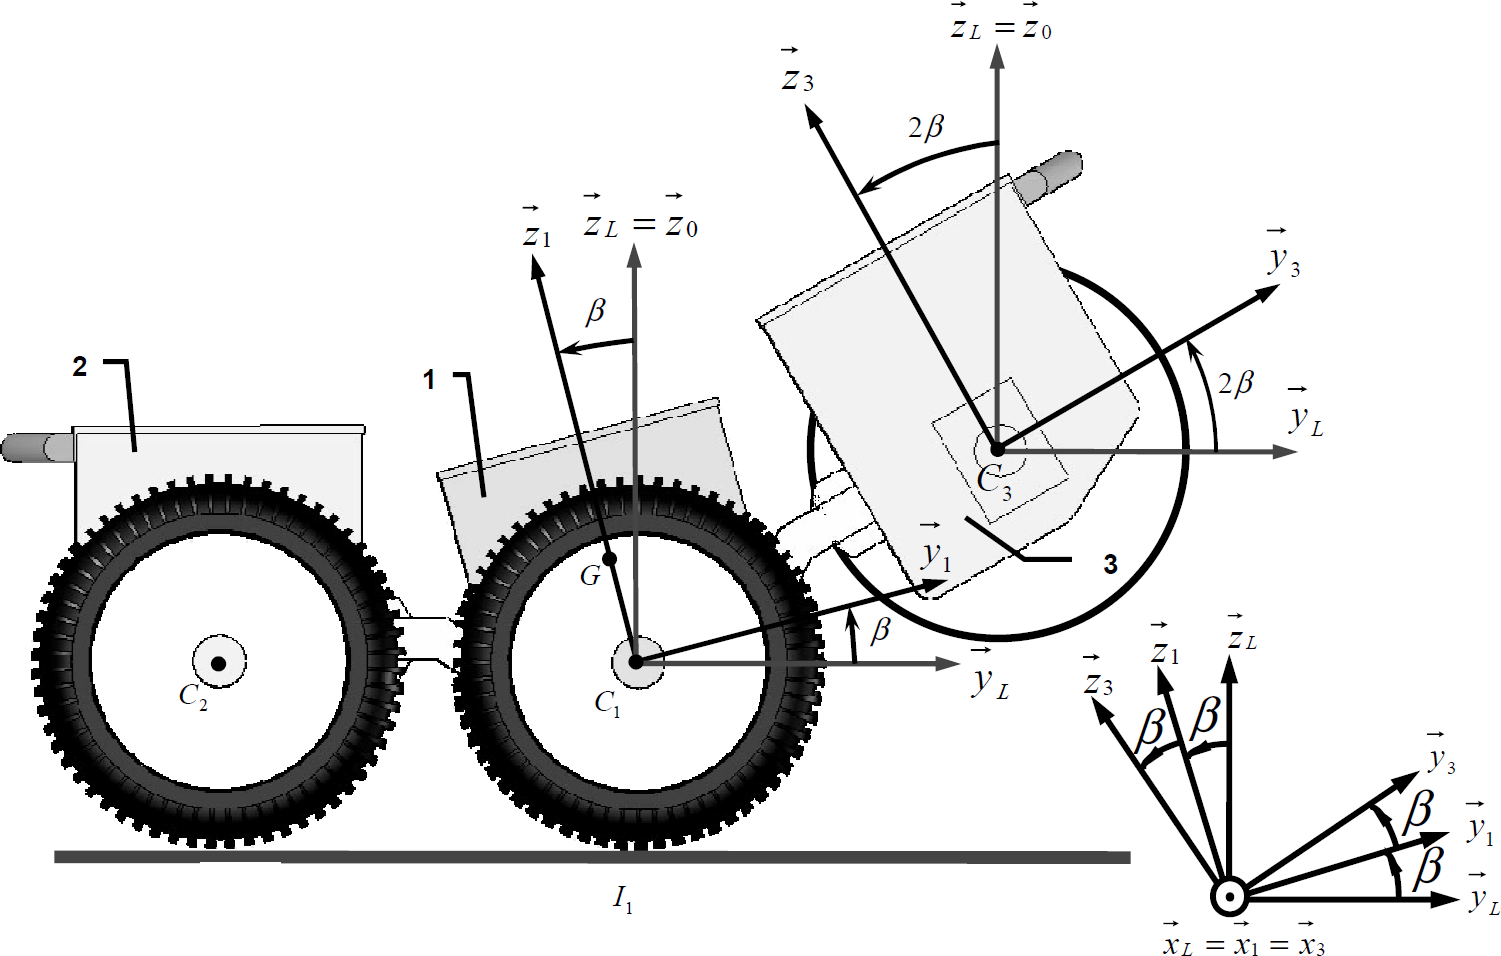
\includegraphics[width=\linewidth]{fig_01_a}
%\textit{Paramétrage}
\end{center}


\begin{center}
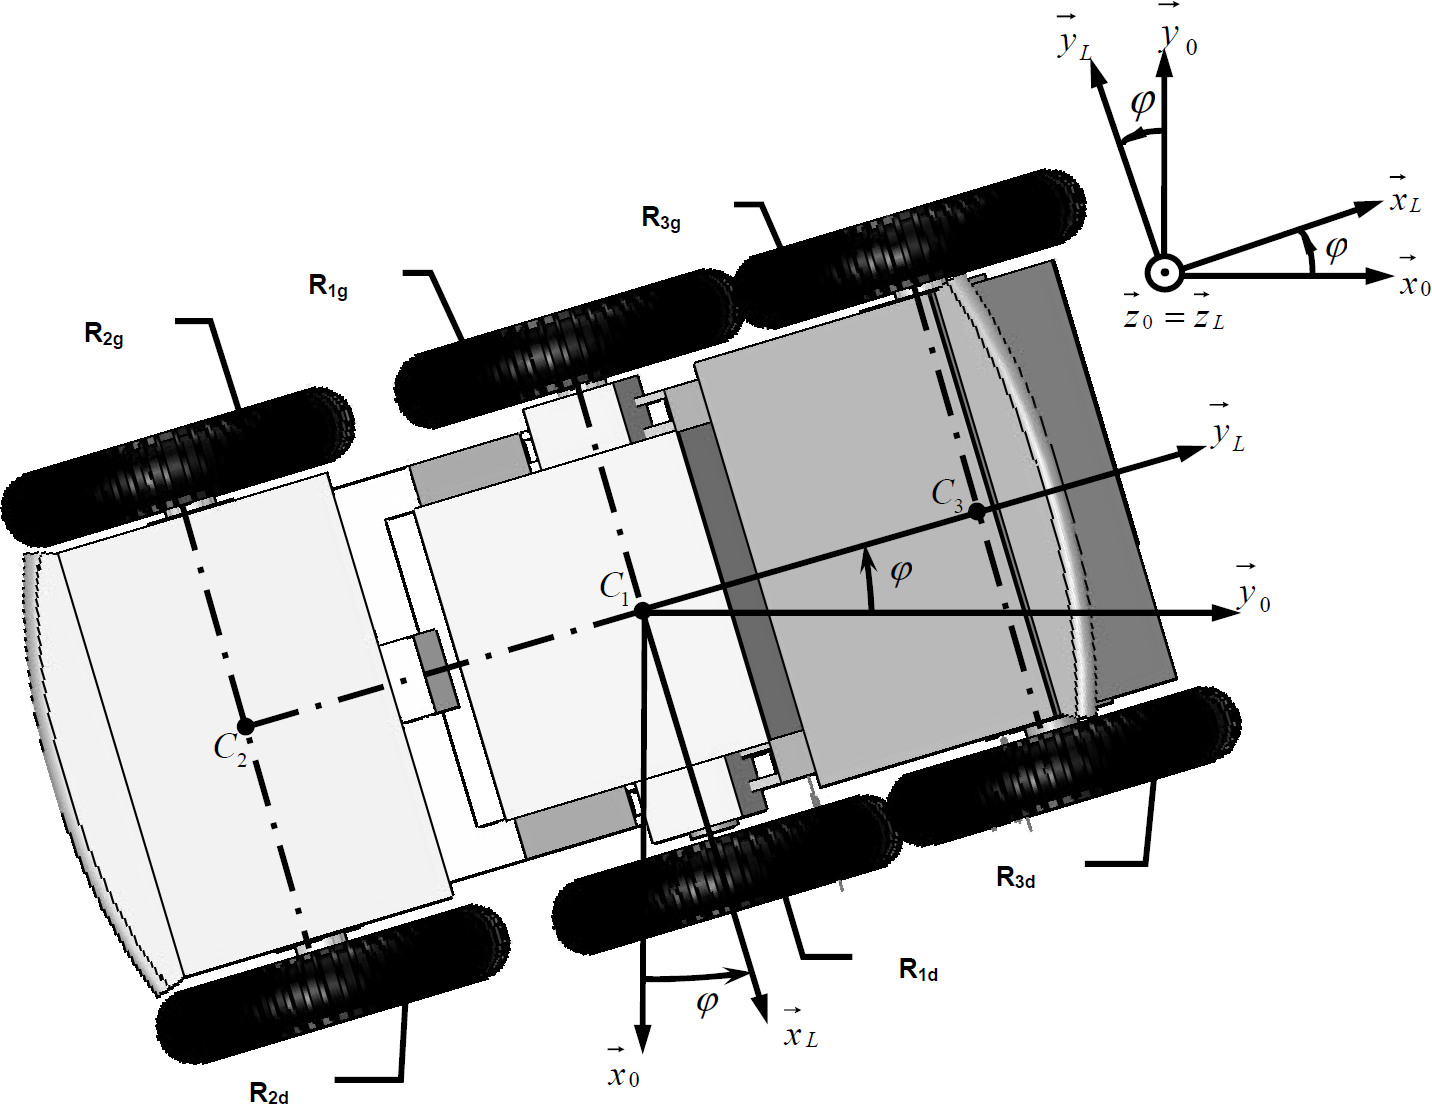
\includegraphics[width=\linewidth]{fig_01_b}
%\textit{Paramétrage}
\end{center}

L’objectif de cette partie est de valider l’aptitude du système à respecter la
loi de vitesse de la figure suivante.

\begin{center}
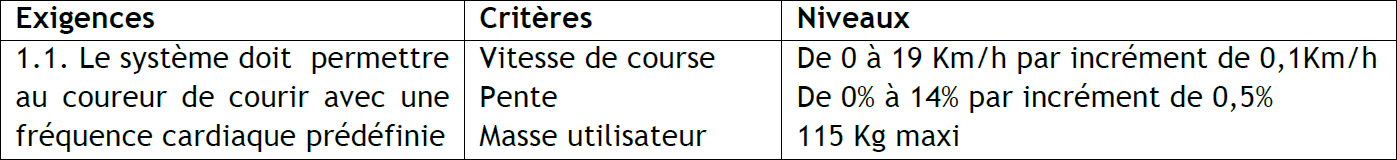
\includegraphics[width=.6\linewidth]{fig_02}
%\textit{Paramétrage}
\end{center}


Les roues centrales et les roues arrière sont en contact avec le sol. Dans ce
mode, seules les roues centrales $R_{1d}$ et $R_{1g}$ sont motrices. Elles roulent
sans glisser sur le sol en $I_{1d}$ et $I_{1g}$. Les roues du pode avant \textbf{3} et du pode
arrière \textbf{2} sont bloquées .


\begin{center}
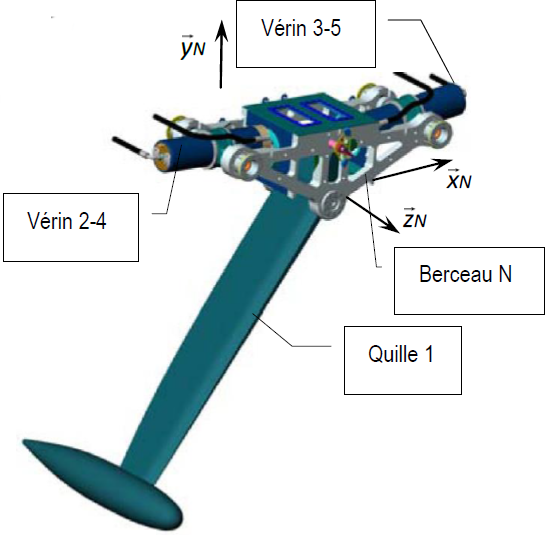
\includegraphics[width=.7\linewidth]{fig_03}
%\textit{Paramétrage}
\end{center}


\begin{center}
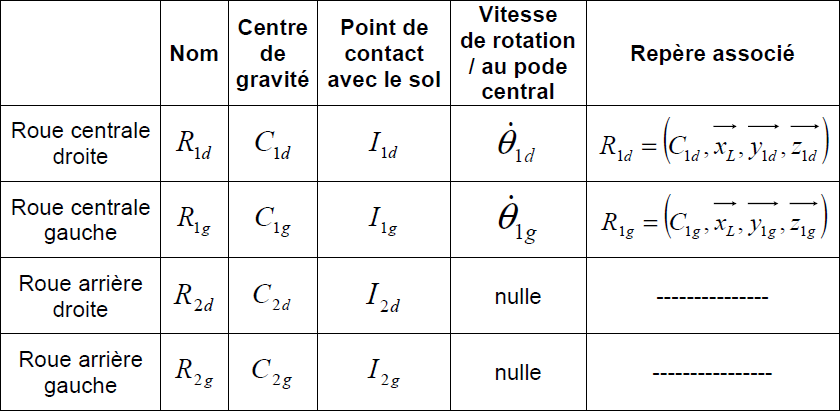
\includegraphics[width=\linewidth]{fig_04}
%\textit{Paramétrage}
\end{center}

\subsubsection*{Paramétrage}%: (annexe 9)
\begin{itemize}
\item $\rep{0}=\repere{O_0}{x_0}{y_0}{z_0}$ lié au sol \textbf{0} supposé galiléen;
\item $\rep{L}=\repere{C_1}{x_L}{y_L}{z_L}$ lié à la plate-forme \textbf{PF} tel que $\varphi=\angl{x_0}{x_L}=\angl{y_0}{y_L}$ appelé angle de lacet;
\item $\rep{1}=\repere{C_1}{x_1}{y_1}{z_1}$ lié au pode central \textbf{1} tel que $\beta=\angl{y_L}{y_1}=\angl{z_L}{z_1}$; $\beta$ est l'angle de tangage; $\beta=2\degres$ (supposé constant pendant tout le mouvement du lacet);
\item $\rep{3}=\repere{C_3}{x_3}{y_3}{z_3}$ lié au pode avant \textbf{3} tel que $2\beta=\angl{y_L}{y_3}=\angl{z_L}{z_3}=4\degres$; 
\item $\vect{C_1C_3}=b\vect{y_3}$ et $\vect{C_1C_2}=-b\vect{y_L}$ avec $b=\SI{553}{mm}$; 
\item la figure précédente permet de définir le paramétrage de chacune des roues de la plate-forme en contact avec le sol avec l’exemple de la roue centrale droite $R_{1d}$.
\end{itemize}

\subsubsection*{Caractéristiques géométriques et d’inertie des solides}
Le mouvement de roulis étant nul et le mouvement de tangage étant fixé à une valeur constante, il est possible de
définir l’ensemble rigide $\Sigma$ constitué des trois podes \textbf{1}, \textbf{2} et \textbf{3}, des deux roues avant, des deux roues arrière et des
bras d’articulation \textbf{4} et \textbf{4’}. Pour chaque constituant de cet ensemble, la masse est supposée répartie
uniformément.
Centre de gravité de $\Sigma$ : $G$ tel que $\vect{C_1G}=a_G\vect{z_1}$ et $a_G=\SI{85}{mm}$, $m_{\Sigma}=\SI{152}{kg}$, $\inertie{C_1}{\Sigma}=\matinertie{A}{B}{C}{0}{0}{0}{\base{x_1}{y_1}{z_1}}$ 	avec $A=\SI{30,2}{kg.m^2}$, $B=\SI{8,2}{kg.m^2}$ et $C=\SI{32,3}{kg.m^2}$.


Roue droite ou gauche + axe de roue : $R_{\text{i d ou g}}$ ($i$ correspond au numéro du pode).
Centre de gravité de $R_{\text{i d ou g}}$ : $C_{\text{i d ou g}}$ tel que l'entraxe ${C_{ig}C_{id}}=2e$, $\vect{C_{i}C_{id}}=e\vect{x_L}$ et $\vect{C_{i}C_{ig}}=-e\vect{x_L}$
avec $e=\SI{340}{mm}$, $m_{r}=\SI{4}{kg}$, rayon d'une roue $R=\SI{225}{mm}$, $\inertie{C_{\text{i d ou g}}}{R_{\text{i d ou g}}}=\matinertie{A_r}{B_r}{B_r}{0}{0}{0}{\base{x_L}{-}{-}}$ valable dans toute base orthonormée directe contenant $\vect{x_L}$ avec $A_r=\SI{0,1}{kg.m^2}$ et $B_r=\SI{0,04}{kg.m^2}$.


Axe des moteurs du pode central : les deux motoréducteurs centraux sont constitués chacun d’un moteur à courant continu alimenté en \SI{48}{V} associé à un réducteur épicycloïdal de rapport de réduction $k = 1/ 25$. La matrice d’inertie en $C_1$ d’un axe moteur droit $M_{1d}$ ou $M_{1g}$ (en rotation suivant $\axe{C_1}{x_L}$) est :
$\inertie{C_{1}}{M_{1d}\text{ ou } M_{1g}}=\matinertie{A_m}{B_m}{B_m}{0}{0}{0}{\base{x_L}{-}{-}}$
avec $A_m=\SI{795e-7}{kg.m^2}$ et $B_m=\SI{8e-3}{kg.m^2}$.

Les masses et inerties des autres pièces seront négligées.

\subsubsection*{Modélisation du contact roue / sol}

Les roues centrales $R_{\text{1d}}$ et $R_{\text{1g}}$ sont motrices, elles roulent sans glisser aux points de contact $I_{1d}$ et $I_{1g}$. On pose $\vect{C_{1d}I_{1d}}=-R\vect{z_L}$ et $\vect{C_{1g}I_{1g}}=-R\vect{z_L}$. 
Le contact avec le sol \textbf{0} est modélisé par le torseur suivant : 
$\torseurstat{T}{0}{R_{\text{1d}}}=\torseurl{\vectf{0}{R_{\text{1d}}} =Y_{\text{1d}}\vect{y_L}+Z_{\text{1d}}\vect{z_L} }{\vect{0}}{I_{\text{1d}}}$ et
$\torseurstat{T}{0}{R_{\text{1g}}}=\torseurl{\vectf{0}{R_{\text{1g}}} =Y_{\text{1g}}\vect{y_L}+Z_{\text{1g}}\vect{z_L} }{\vect{0}}{I_{\text{1g}}}$ .


Les roues arrière $R_{\text{2d}}$ et $R_{\text{2g}}$ sont bloquées, leur vitesse de rotation par rapport au pode arrière \textbf{2} est nulle. Le
contact avec le sol \textbf{0} est modélisé par le torseur suivant :
$\torseurstat{T}{0}{R_{\text{2d}}}=\torseurl{\vectf{0}{R_{\text{2d}}} =T_{\text{2d}}\vect{n_g}+Z_{\text{2d}}\vect{z_L} }{\vect{0}}{I_{\text{2d}}}$ et
$\torseurstat{T}{0}{R_{\text{2g}}}=\torseurl{\vectf{0}{R_{\text{2g}}} =T_{\text{2g}}\vect{n_g}+Z_{\text{2g}}\vect{z_L} }{\vect{0}}{I_{\text{2g}}}$  avec 
$\vect{n_d}$ et $\vect{n_g}$
deux vecteurs unitaires opposés aux vitesses de glissement des roues $R_{\text{2d}}$ et $R_{\text{2g}}$ par rapport au sol 
\textbf{0} respectivement en $I_{\text{2d}}$ et $I_{\text{2g}}$.
On pose $\vect{C_{\text{2d}}I_{\text{2d}}}=-R\vect{z_L}$
et $\vect{C_{\text{2g}}I_{\text{2g}}}=-R\vect{z_L}$.
$T_{\text{2d}}=fZ_{\text{2d}}$ et $T_{\text{2g}}=fZ_{\text{2g}}$; $f$ est le facteur de frottement constant au contact roue/sol $f=0,6$.

\subsubsection*{Autres liaisons}

Toutes les autres liaisons de la plate-forme sont supposées parfaites (sans jeu, sans frottement).

\subsubsection*{Motoréducteur centraux}


L’action mécanique développée par le motoréducteur sur la roue centrale droite $R_{\text{1d}}$ est notée
$\torseurstat{T}{\text{moteur}}{R_{\text{\text{1d}}}}
=\torseurl{\vect{0}}{-C_m\vect{x_L}}{C_1}$.

L’action mécanique développée par le motoréducteur sur la roue centrale droite $R_{\text{1g}}$ est notée
$\torseurstat{T}{\text{moteur}}{R_{\text{\text{1g}}}}
=\torseurl{\vect{0}}{C_m\vect{x_L}}{C_1}$.


\fi


\subparagraph{}\textit{Justifier la forme de la matrice d’inertie de l’ensemble $\Sigma$ au point $C_1$ dans la base $\base{x_1}{y_1}{z_1}$.}
\ifprof
\begin{corrige}
\end{corrige}
\else
\fi


Dans un premier temps, l’objectif est de déterminer la somme des efforts normaux $Z_{\text{2d}} + Z_{\text{2g}} $ s’exerçant sur les roues arrières. Isolons l’ensemble de la plate-forme PF, soit l’ensemble $\Sigma$, les roues centrales et les  motoréducteurs.
Plaçons-nous dans le plan médian $\left( C_1, \vect{y_L}, \vect{z_L}\right)$ de la plate-forme PF . Nous définissons le projeté $I_1$ des points de
contact $I_{\text{1d}}$ et $I_{\text{1g}}$ dans ce plan. $I_1$ est défini par le vecteur : $\vect{C_1I_1}=-R\vect{z_L}$. D’autre part, nous avons 
$\vect{C_2I_1}=b\vect{y_L}-R\vect{z_L}$ et $\vect{C_3I_1}=-b\vect{y_3}-R\vect{z_L}$.
Nous ferons l’hypothèse que le moment dynamique $\vectmd{I_1}{PF}{0} \cdot \vect{x_L}$
est négligeable devant les actions mécaniques.




\subparagraph{}\textit{
En appliquant le théorème du moment dynamique à la plate-forme PF en mouvement par rapport au
référentiel galiléen $\rep{0}$ en $I_1$ en projection sur $\vect{x_L}$, déterminer l’expression littérale de la somme des efforts normaux de contact $Z_{\text{2d}} + Z_{\text{2g}} $, entre les roues arrière et le sol. Réaliser l’application 
numérique et comparer la valeur obtenue à la somme des efforts normaux s’exerçant sur les roues arrière lorsque la plate-forme est immobile en appui sur ses six roues sur un sol plan, à savoir $\left(Z_{\text{2d}} + Z_{\text{2g}} \right)_{\text{Repos}}=\left( m_2+2m_r\right)g$
avec $m_2 = \SI{52}{kg}$ la masse du pode arrière \textbf{2}.}
\ifprof
\begin{corrige}
\end{corrige}
\else
\fi

L’objectif est dans un second temps de valider l’aptitude des moteurs à suivre la loi de vitesse en lacet exigée. Il est
proposé de déterminer l’expression du couple moteur $C_m$ par une approche énergétique.


\subparagraph{}\textit{Déterminer l’énergie cinétique galiléenne de l’ensemble des solides en mouvement. Le résultat sera mis sous la forme  $\dfrac{1}{2} J \dot{\varphi}^2$ où $J$ est à exprimer sous forme littérale en fonction des données du problème.}
\ifprof
\begin{corrige}
\end{corrige}
\else
\fi

\subparagraph{}\textit{Mettre en \oe{}uvre le théorème de l’énergie cinétique afin de déterminer l’expression du couple moteur. Vous 
donnerez le résultat sous la forme 
$C_m = k_2\left(J\ddot{\varphi}+k_1 \left(T_{\text{2d}} + T_{\text{2g}} \right)\right)$
où $k_1$ et $k_2$ sont à exprimer sous forme
littérale en fonction des données du problème.
Vous veillerez à bien faire apparaître les différentes étapes
de votre raisonnement et à fournir des expressions littérales.}
\ifprof
\begin{corrige}
\end{corrige}
\else
\fi

Pour la question suivante, vous prendrez $J =\SI{34}{kg.m^2}$, $k_1=\SI{0,65}{m}$ et $k_2=1,3\times 10^{-2}$ sans unité.


\subparagraph{}\textit{Calculer le couple moteur maximal : $C_m$ maxi. À partir du graphe de fonctionnement du moteur, conclure quand à l’aptitude de la motorisation à générer le mouvement de lacet désiré.}
\ifprof
\begin{corrige}
\end{corrige}
\else
\fi


\begin{center}
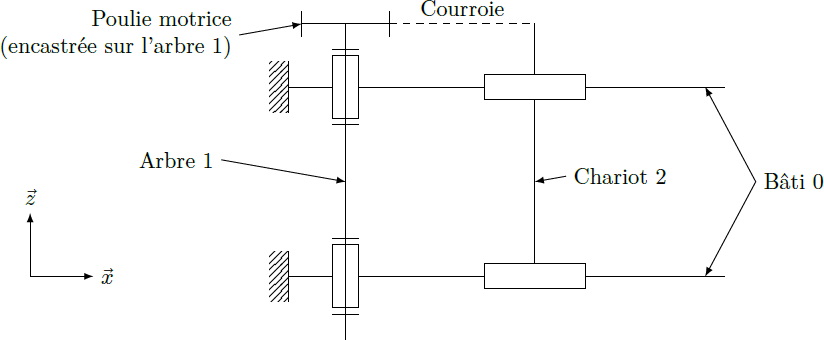
\includegraphics[width=\linewidth]{fig_05}
%\textit{Paramétrage}
\end{center}

\ifprof
%\end{multicols}
\else
\end{multicols}
\fi


